\chapter{Trabalhos Relacionados}\label{ch:Relacionados}


O Abuso Sexual Infantil (ASI) maninesta-se como um problema global. Diante disso, profissionais da saúde e pesquisadores passaram a se dedicar a compreender as raízes  deste mal que assola milhares de crianças todos os anos \cite{deslandes1994atenccao, dahlberg2006violencia, da2017violencia}. A área de criminologia em específico, desenvolveu uma série de teorias acerca das causas para os atos infracionais. Dentre elas, destaca-se a Teoria da Atividade Rotineira, ilustrada na \autoref{fig:Crime}.
%Inúmeros métodos surgiram para compreender as raízes do problema, dentre eles, cita-se a Análise de Causa Raiz (ACR). Tal método visa descobrir a causa de um problema para identificar soluções adequadas \cite{rooney2004root}.


\begin{figure}[htb]
    \begin{minipage}{0.45\textwidth}
      \hspace{35pt} O infográfico da \autoref{fig:Crime} apresenta os três elementos básicos da Teoria da Atividade Rotineira, também conhecida como de Triângulo do Crime. Em resumo, três elementos são considerados essenciais para a ocorrência de um crime. Para que um crime aconteça deve-se haver um criminoso motivado sem supervisão, um lugar sem fiscalização e um vítima desprotegida ou vulnerável. Tomar atitudes preventivas sob qualquer um destes elementos, dificulta a ocorrência do crime. Todavia, destaca-se que estes elementos não possuem pesos iguais, mas sim, se interbalanceiam entre si. Em certas condições, um lugar muito bem fiscalizado poderia não ser um empecilho para um criminoso muito motivado.
    \end{minipage}
    \begin{minipage}{0.55\textwidth}
      \caption{\label{fig:Crime}Triângulo do Crime}
      \begin{center}
        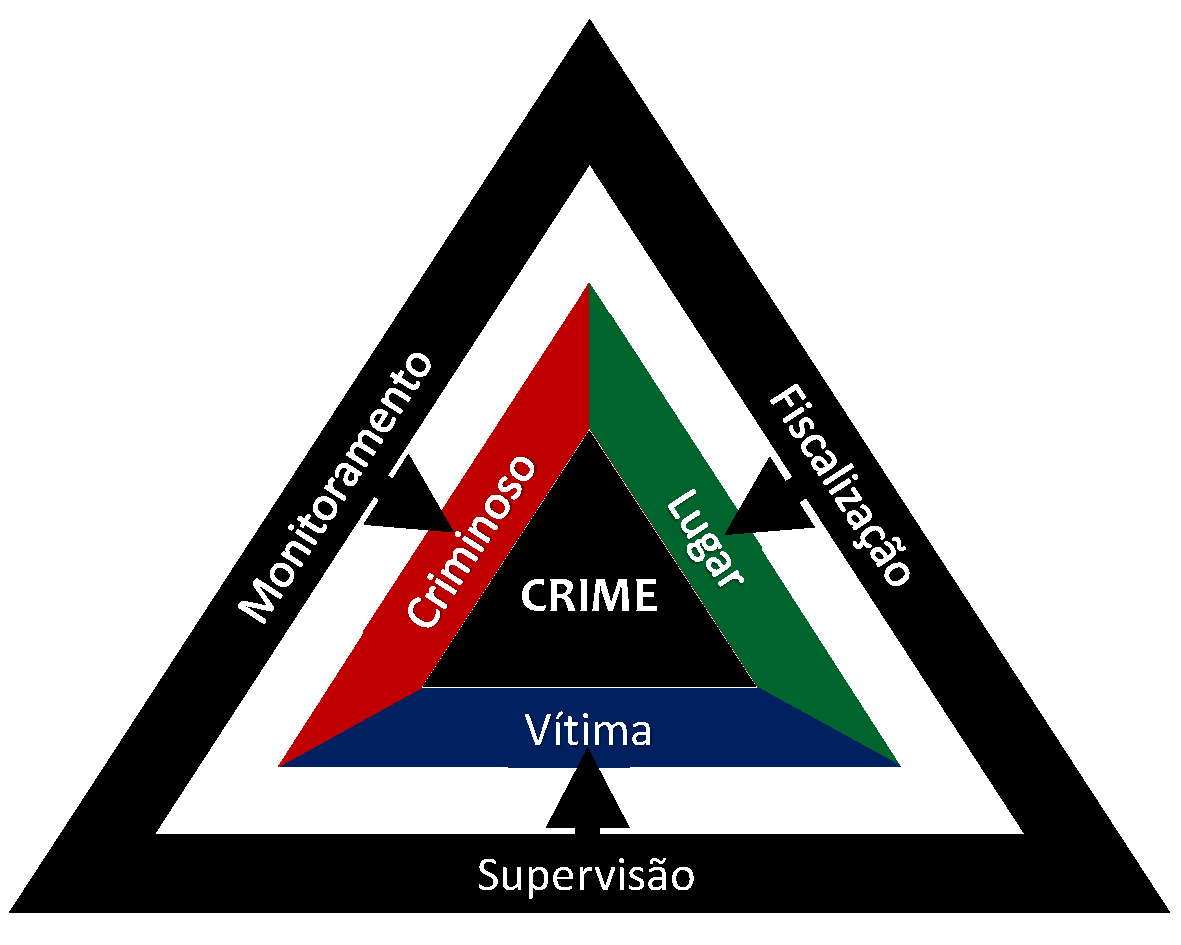
\includegraphics[width=\linewidth]{./Figuras/TrianguloCrime.pdf}
      \end{center}
      \legend{Fonte: os autores}
    \end{minipage}
\end{figure}

%criminoso = supervisão
%lugar = fiscalização
%Vítima = proteção

O Triângulo do Crime apresenta as três partes fundamentais para a ocorrência de um crime. As estratégias de combate ao abuso sexual infantil se objetivam a agir sob estas partes fundamentais. Algumas estratégias são focadas no monitoramente de criminosos\footnote{\label{note:nota1}Círculos de Suporte e Responsabilidade (Em inglês: Circles of Accountability and Support - CoSA) são grupos de voluntários com supervisão profissional para apoiar os agressores sexuais à medida que se reintegram à sociedade após serem libertados do encarceramento.}, outras no fortalecimento da fiscalização em espaços públicos ou privados\footnote{Lei nº 12.038, de 1º de outubro de 2009 dificulta a exploração sexual de crianças e adolescente impossibilitando a hospedagem deles por terceiros que não apresentem autorizações legais.}, e outras na capacitação preventiva de potenciais vítimas, tornando-as menos vulneráveis\footnote{O programa educacional Talking about Touching é um programa focado no ensino de habilidades básicas para crianças com finalidade de ajudá-las a se protegerem de situações abusivas.}. Cada estratégia pode ser dividida com base em seus níveis de prevenção. Os níveis de prevenção são apresentados em maiores detalhes na \autoref{fig:prevencao}.

\begin{figure}[htb]
	\caption{\label{fig:prevencao}Níveis de Prevenção}
  \begin{center}
    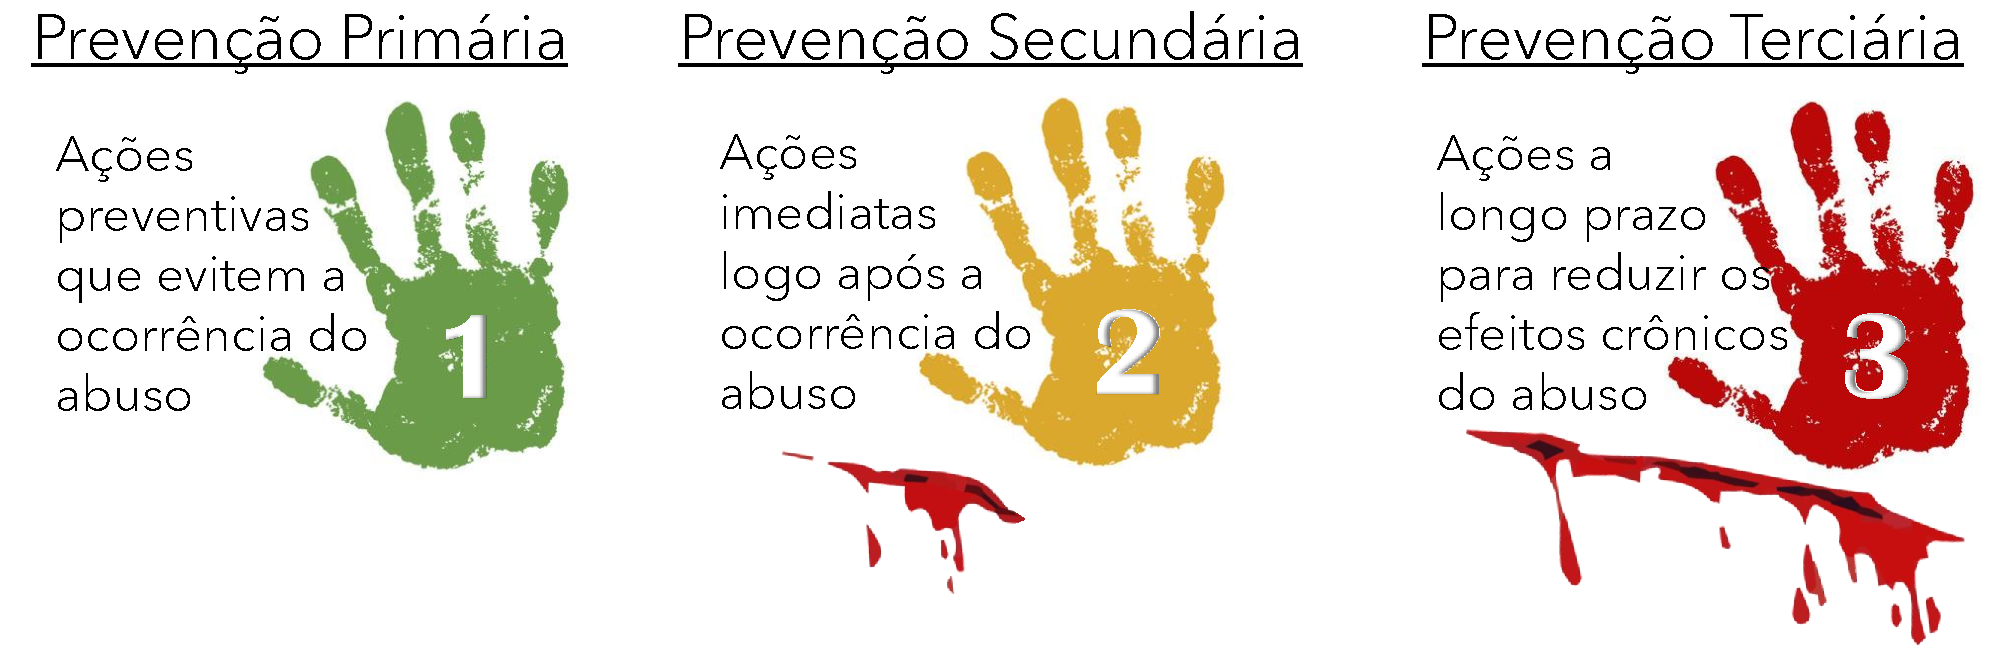
\includegraphics[width=\linewidth]{./Figuras/Prevencao.pdf}
	\end{center}
	\legend{Fonte: os autores}
\end{figure}

A \autoref{fig:prevencao} apresentada os três níveis de prevenção mais comumentes relatados na literatura pesquisada. São eles: prevenção primária, prevenção secudária e prevenção terciária \cite{dahlberg2006violencia, santos2011guia, maria2012abusos}. No caso do abuso sexual infantil, a prevenção primária engloba iniciativas que antecipam a incidência do abuso sexual contra crianças e adolescentes  \cite{marcelino2017vamos}. A prevenção secundária enfatiza uma resposta imediata após a ocorrência da violência sexual. Já a prevenção terciária corresponde, de modo geral, a ações de longo prazo para o tratamento e recuperação das vítimas \cite{people2020expert}. Informa-se que a literatura médica relata também um quarto nível de prevenção. A prevenção quartenária descreve sobre ações preventivas contra eventuais exageros na utilização de métodos preventivos \cite{tesser2017importante}. Embora presente na literatura médica, salienta-se que a atual dissertação engloba apenas os três níveis de prevenção mais relatados pela bibliografia pesquisada acerca do abuso sexual infantil.

Os níveis de prevenção do abuso sexual infantil não se resumem a atuar apenas sob as crianças. Há registros de prevenção terciária relacionados inclusive ao tratamento/acompanhamento de agressores sexuais\footref{note:nota1}. O combate ao abuso sexual infantil assume então inúmeras facetas, cada qual, objetivada a diminuir de alguma forma os fatores de risco que influênciam a ocorrência de violações sexuais.

Os Fatores de Risco são aquelas circunstâncias que aumentam a probabilidade da ocorrência de um episódio de violência. Deste modo, o abuso infantil apresenta mais chances de ocorrer quando os fatores de risco se acumulam. Os Fatores de Risco interagem entre si, no que é chamado de risco em cascata, no qual um risco inicial pode acompanhar ou desencadear outros riscos, terminando por resultar em um acúmulo sucessivo de fatores de risco \cite{Recommendations2019Taylor}. A \autoref{fig:Riscos} apresenta a disposição dos fatores de riscos mais apontados pela literatura na área. 

%O modelo socio-ecológico é uma estrutura de saúde pública desenvolvida pelos Centros de Controle e Prevenção de Doenças (em inglês: Centers for Disease Control and Prevention - CDC) \cite{centers2019social}. O modelo socio-ecológico data desde a década de 1970, sendo  aplicado aos casos de abuso infantil \cite{dahlberg2006violencia}. O modelo explora a relação entre os fatores individuais e contextuais e considera a violência como produto dos múltiplos níveis de influência sobre o comportamento


%https://www.scielo.br/pdf/csc/v11s0/a07v11s0.pdf \cite{dahlberg2006violencia}

%https://www.unicef.org/media/66741/file/Promising-programme-responses.pdf4 \cite{topromising}

%https://www.k12.wa.us/sites/default/files/public/hivsexualhealth/pubdocs/Erin%27s%20Law%20Report.pdf [fez que nem eu] \cite{Recommendations2019Taylor}

%https://www.doh.wa.gov/Portals/1/Documents/Pubs/140-165-SexualViolencePreventionPlan.pdf [fez que nem eu] \cite{sexual2017department}

%https://www.cdc.gov/violenceprevention/pdf/svprevention-a.pdf \cite{centers2004sexual}

\begin{figure}[htb]

	\caption{\label{fig:Riscos}Modelo Ecológico}
  \begin{center}
    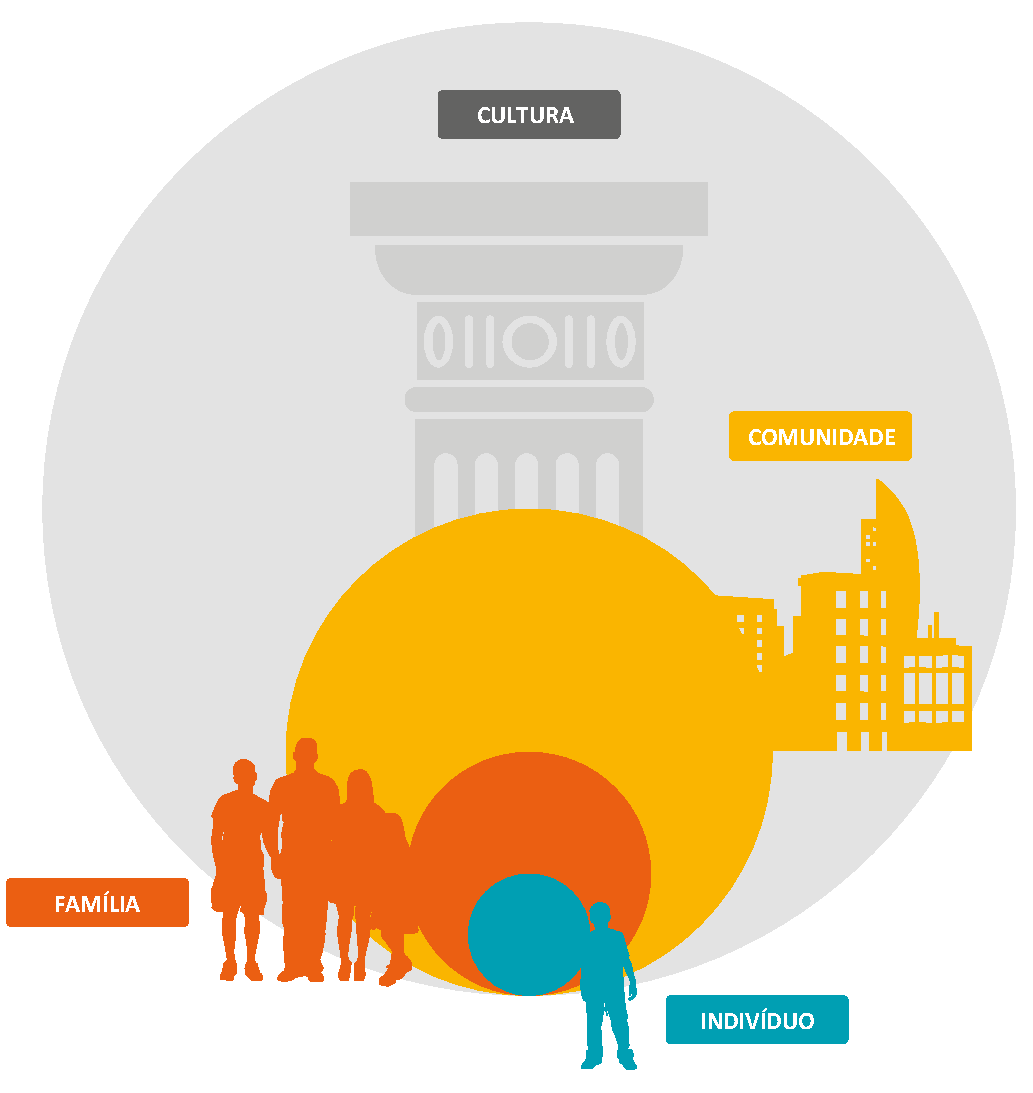
\includegraphics[width=0.8\linewidth]{./Figuras/FatoresRisco.pdf}
	\end{center}
  \legend{Fonte: adaptado de \cite{blasco2018abuso}}

\end{figure}
%https://www.savethechildren.es/sites/default/files/imce/docs/mas_me_duele_a_mi.pdf
%[ainda sita-se a falta de sensibilização da sociedade, lideres politicos, etc tec.... pag 39]

O infográfico da \autoref{fig:Riscos} ilustra os quatro fatores de risco do Modelo Ecológico. Salienta-se os fatores de risco podem váriar em quantidade e em nomenclatura, dependendo da lituratura pesquisa \cite{centers2004sexual, sexual2017department, blasco2018abuso, topromising}. Todavia, a ideia base do Modelo Ecológico tendem a permanecer inalterada. O modelo em si, explora a relação entre os fatores individuais e contextuais que acabam por implicar em um cenário de violência \cite{dahlberg2006violencia}. Os fatores de risco mais influentes são:

\begin{itemize}
  \item \textbf{Indivíduo:} \hfill Aspectos individuais que fomentem a ocorrência do abuso sexual. %Válido tanto para as vítimas quanto para os agressores. 
  \item \textbf{Família:} \hfill Questões familiares que viabilizam as condições para a violência.  %circunstâncias
  \item \textbf{Comunidade:} Condições econômicas e governamentais que propiciem o abuso.
  \item \textbf{Cultura:} \hfill Crenças sociais que estimulem atividades sexuais com menores. 
\end{itemize}


se aplica tanto a vítima quanto ao agressor. este nível do modelo ecológico  ocaliza as características do indivíduo que aumentam a probabilidade de ele ser vítima ou agressor



[A culturas que encorajam o casamento infantil]
[A sociedades que acreditam que ao se relacionarem com crianças estão se limpando da AIDS]


--------------------------------


O atual capítulo busca elencar as principais iniciativas relatadas pela literatura pesquisada no combate ao abuso sexual infantil. Deste modo, a seção 1 fala das estrategais tais, a seção 2 fala das estrategias aquelas, a seção..... seção 10 aborda em maiores detalhes as estrategias que utilizam jogos, sendo este o foco principal deste trabalho. 

um levantamento bibliográfico das principais estratégias de combate ao abuso sexual infantil foi realizado, com ênfase nas estratégias que envolvem jogos \cite{wazlawick2017metodologia}


[o livro] relata que para tratar um problema, antes é nessário ter uma visão geral de todos os metódos já documentados que tentaram tratar o problema em questão. Deste modo, as principais estratégias que combate a violência sexual infantil encontradas na literatura são elencadas por esta pesquisa. A seção 1.. bla bla bla..


Esta seção apresenta os trabalhos relacionados, bem como o estado da arte. Os trabalhos foram selecionados de acordo com sua contribuição para as áreas de: sistemas colaborativos, design participativo, dispositivos de alta tecnologia e Comunicação Aumentativa e Alternativa.

Este Cap´ıtulo apresenta a revis˜ao da literatura realizada para obter a compreens˜ao geral do estado da arte e as limita¸c˜oes das metodologias existentes para avalia¸c˜ao de jogos. Foram pesquisados artigos nos motores de busca: SciELO, Google Acadˆemico, CAPES. Tamb´em foram pesquisados: peri´odicos; livros e sites de referˆencia que descrevem jogos avaliados, recomenda¸c˜oes no desenvolvimento de jogos e metodologias de an´alise de jogos s´erios; al´em de consultadas as referˆencias citadas nesse trabalho. 

As se¸c˜oes deste Cap´ıtulo dividem os artigos em grupos com base no foco do jogo avaliado. Jogos destinados ao treinamento de profissionais adultos acerca de determinado tema est˜ao condensados na se¸c˜ao 3.1. Jogos de lazer, sem nenhum nicho et´ario espec´ıfico s˜ao apresentados na se¸c˜ao 3.2. Jogos focados na ensino-aprendizagem de adolescentes e jovens adultos s˜ao tratados na se¸c˜ao 3.3 e jogos com o intuito de ensinar e educar crian¸cas est˜ao condensados na se¸c˜ao 3.4. A se¸c˜ao 3.5 condensa os conhecimentos adquiridos na revis˜ao bibliogr´afica sobre os m´etodos de avalia¸c˜ao de jogos. Ao final, a se¸c˜ao 3.6 lista diretrizes e orienta¸c˜oes para o desenvolvimentos de jogos, jogos s´erios e materiais did´aticos infantis. [serão abordados as princiapis formas de combate a volência sexual infantil com ênfase nas estrategias que envolvem jogos (JOGO SÉRIO) ]

Por serem os jogos aplicados a contextos sérios uma área recente (DJAOUTI et al., 2011) e dado o interesse desta pesquisa na busca por métodos de game design, com foco mais teórico do problema, usou-se uma estratégia “top-down” de abordagem, com a execução de um mapeamento sistemático (PETERSEN et. al., 2008) para levantar inicialmente os dados quantitativos da área. Foram utilizados os seguintes mecanismos de busca acadêmica (MBAs): ACM DL, IEEExplore, Science Direct, Pubmed e Web of Science. A escolha por esses MBAs deu-se por abrigarem publicações de qualidade reconhecida pela Coordenação de Aperfeiçoamento de Pessoal de Nível Superior (CAPES) (CAPES, 2016) e por possuírem a maior quantidade de recursos de busca e seleção (BUCHINGER et al., 2014).

Nos últimos anos a demanda e produção de JS vem aumentando, tanto quanto para os JSA que, com a evolução da tecnologia, dispõem de cada vez mais recursos para torná-los viáveis (VAN DIEST et al., 2013). Dessa forma, descreve-se na seção 3.1 uma pesquisa bibliográfica sistemática na qual foram analisados trabalhos que propõe JSA para reabilitação do equilíbrio. A seção 3.2 descreve exemplos de JSA desenvolvidos para reabilitação do equilíbrio dinâmico que estão ordenados por data de publicação. A seção 3.3 compara e discute os JSA encontrados na revisão bibliográfica.


Como o foco da pesquisa é o uso de Jogos Sérios para Alfabetização Matemática, principalmente no que diz respeito ao ensino dos elementos ou habilidades cognitivas que fazem parte do estágio fundamental, realizaram-se dois mapeamentos sistemáticos da literatura nacional em busca de artigos publicados em eventos e revistas científicas que pudessem abordar este tema.

3.0 Tomando como base o foco desta pesquisa na interação competitiva-colaborativa em Jogos Sérios e a temática proposta (dengue), foram realizadas pesquisas com o intuito de encontrar trabalhos que envolvessem conjuntamente estes aspectos. Um jogo com estas características (JSCC sobre dengue) porém, não foi encontrado. Dessa forma, foram propostas duas atividades: realizar uma Revisão Sistemática de Literatura sobre JSCC, e realizar uma pesquisa por experiência sobre iniciativas que abordem o tema dengue. 

3.1
Inicialmente foi realizado um Mapeamento Sistemático de Literatura sobre JSCC – pesquisa completa publicada em evento nacional (BUCHINGER; HOUNSELL, 2013) – considerando o período entre 2003 a 2013 e utilizando-se de seis mecanismos de busca acadêmicos (MBAs): ACM Digital Library15, IEEE Xplore16, Science Direct17, Scopus18 e Web of Knowledge/Science19. Numa primeira tentativa, considerando as flexões gramaticais das palavras chaves (através de caracteres coringas), foi definida a seguinte frase de busca: (“serious game*”) AND (collaborat*) AND (compete OR competi*)

Enfatiza-se o critério utilizado para o termo competição. Foram utilizados dois termos: um fixo, para incluir a palavra competir (compete), mas não variantes que possuem outro sentido e se apresentam com o mesmo prefixo (e.g. competence ou competency); e outro flexível para abranger algumas variantes do termo competição (e.g. competition e competitive)....


----------------





%procurando aumentar o conhecimento dos menores na problemática em questão, tornando-as mais resilientes e menos vulneráveis

%, visando mitigar os males iniciais causados por um evento de abuso


%https://repositorio.ufscar.br/bitstream/handle/ufscar/2835/TeseMGSP.pdf?sequence=1&isAllowed=y

%https://www.udesc.br/arquivos/cct/id_cpmenu/1024/disserta_ao_completa_15532596804969_1024.pdf

%https://www.scielo.br/pdf/csc/v11s0/a07v11s0.pdf

%http://portaldoprofessor.mec.gov.br/storage/materiais/0000016936.pdf

%https://www.scielosp.org/article/csc/1999.v4n1/171-181/pt/

%https://repositorio.iscte-iul.pt/bitstream/10071/15660/1/Disserta%c3%a7%c3%a3oDianaMarcelino.pdf

%https://repositorio.iscte-iul.pt/bitstream/10071/12615/3/2016_ECSH_DPSO_Dissertacao_Magda%20Moita.pdf

%https://repositorio.iscte-iul.pt/bitstream/10071/10673/1/2015_ECSH_DPSO_Dissertcao_Nicole%20Christine%20Alves%20Figueiredo.pdf

%https://www.unicef.org/media/66741/file/Promising-programme-responses.pdf4

%http://repositorio.ispa.pt/bitstream/10400.12/1768/1/TES%20MARI1.pdf

%https://www.k12.wa.us/sites/default/files/public/hivsexualhealth/pubdocs/Erin%27s%20Law%20Report.pdf

%https://www.cdc.gov/violenceprevention/pdf/svprevention-a.pdf

%https://www.doh.wa.gov/Portals/1/Documents/Pubs/140-165-SexualViolencePreventionPlan.pdf

%https://bmcpublichealth.biomedcentral.com/articles/10.1186/s12889-017-4502-6

%https://www.gov.scot/publications/expert-group-preventing-sexual-offending-involving-children-young-people-prevention-responses-harmful-sexual-behaviour-children-young-people/pages/11/

%https://www.e-publicacoes.uerj.br/index.php/sustinere/article/view/30004/23155

%https://www.scielosp.org/article/csc/2006.v11suppl0/1163-1178/pt/

%https://endsexualviolencect.org/what-we-do/prevention/primary-prevention/

%e discutir medidas para sua prevenção
%inúmeras iniativas surgiram no intuito de eliminar este mau que assola milhares de crianças todos os anos. As estratégias de combate e enfrentamento ao abuso sexual infantil 


%\cite{eck1995examining}




%``Na década de 1980, profissionais da saúde como médicos, pesquisadores e os sistemas de  saúde  pública  passaram  a  se  dedicar  a  compreender  as  raízes  daviolência  e  discutir medidas   para   sua   prevenção.   É   também   nessa   década   que   a   violência   passa   a   ser considerada  um  problema  de  saúde  pública,  devido  ao  aumento  de  mortes  e  traumas  que congestionam os serviços de saúde (DESLANDES, 1994; DAHLBERG e KRUG, 2007).'' %https://www.e-publicacoes.uerj.br/index.php/sustinere/article/view/30004/23155






\newpage

\section{Teste $
\includegraphics[width=0.05\linewidth]{./Figuras/Prevencao1.pdf}$$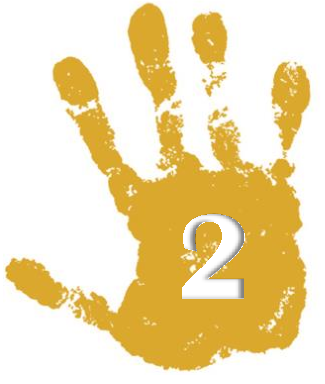
\includegraphics[width=0.05\linewidth]{./Figuras/Prevencao2.pdf}$$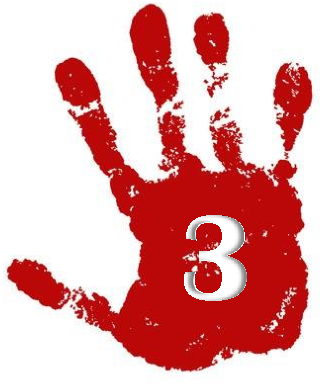
\includegraphics[width=0.05\linewidth]{./Figuras/Prevencao3.pdf}$}\label{sec:teste}

%\icon{./Figuras/TrianguloCrime.pdf}

É importante lembrar que existe diferença entre ``distinção entre ações governamentais voltadas ao enfrentamento da exploração sexual e ações voltadas à prevenção do abuso sexual.''  \cite{caccia2014conselheiros}

Formas de combate a violência sexual (\textbf{PROGRAMAS [AULAS], EXAMES CLINICOS, OBSERVAÇÕES NO COMPORTAMENTO}):

\begin{itemize}
  \item Criança denuncia avô por abuso após aula sobre violência sexual no Paraná. \cite{central2019crianca} [\textbf{Proerd}, avó acareciava ela]
  \item Criança escreve bilhete após palestra em escola de MT e denuncia pai: 'Já fui abusada pelo meu pai, isso pode ser denúncia?' \cite{lidiane2018crianca} [\textbf{Proerd}, pai abusava ela]
  \item Mãe descobre que filha de 5 anos foi estuprada ao levar menina em pediatra de RO \cite{jonatas2018crianca} [\textbf{Exames de rotina}, medica constatou abuso pelo primo de 13 anos]
  \item Menina denuncia padrasto por estupro após palestra sobre violência sexual, no ES [\textbf{PROERD?}]
\end{itemize}

%REVISAR A CITAÇÃO, PELO QUE PARECE, ESSE TIPO DE CITAÇAO VAI COMO NOTA DE RODAPE E NAO NAS REFERENCIAS... Basta dizer: 'Disponível em: <https://oglobo.globo.com/.......'

Aqui abaixo vemos a \textbf{estratégia da Alemanha} em produzir pornografia infantil falsa:
\begin{itemize}
  \item https://www.zdf.de/nachrichten/heute/lambrecht-will-ermittlern-herstellung-gefakter-kinderpornografie-erlauben-100.html

  \item https://www.dw.com/en/germany-plans-to-use-fake-child-porn-to-snare-pedophiles/a-51361810

  \item https://www.terra.com.br/noticias/alemanha-planeja-usar-pornografia-infantil-falsa-para-capturar-pedofilos,869a166ee7af97bb44f30200b7f93597y5krakph.html
\end{itemize}


\begin{enumerate}
    \item \cite{mendelson2015parent}
  
    \item .[Justice System Restrictions] = ???????????????????
  
    \item .[Advocacy and Media Campaigns] = Campanhas governamentais (Darkness to Light, Stop It Now! e Prevention Project Dunkelfeld)
  
    \item .[Youth-Serving Organizations] => código de conduta????
  
    \item .[School-Based Programs] = AULAS (PROERD)
  
    \item .[Treatment of Offenders] = Gestão de Infratores
  
    \item .[Treatment of Victims] = Tratamento psicológico (centros de tratamento)
    
    \item PROPOSTA DO ARTIGO [Parent-Focused Prevention] = Treinamento de Pais (TP)
  \end{enumerate}

  TRILHA DA PROTEÇÃO: \cite{meyer2017analise}

  ``Existe una gran variedad de opciones metodologicas al alcance de los usuarios. Dentre de estas, las mas utilizadas han sido los \textbf{materiales impresos, los videos o materiales audiovisuales, las charlas, las representaciones teatrales y el role playing}'' (corrigir erros do espanhol) [Esse artigo é bom, pois fala dos toque bons, toque ruins, partes íntimas, etc] ... ``el abusador impone a el nino ley de silencio (segredo)'' ... ``los programas deberian poner el acento en transmitir a los ninos la importancia de divulgar el abuso y no en pedirles que se nieguen y sean capaces de deternerlo'' [LEMBRA DO JOGO TRIALHA DA PROTEÇÃO, ao completar a criança recebe o título de 'PROTEGIDO'] \cite{martinez2011prevencion} 

  
``Assim, as autoras reforçam a importância e a necessidade de os \textbf{professores receberem treinamento especializado} para identificar e intervir nesses casos, já que muitas professoras apresentam apenas um conhecimento superficial sobre o tema, buscam informações em meios não apropriados e não tem clareza sobre os procedimentos que devem tomar'' [Outra estratégia é o treinamento especializado de professores] ``Uso de \textbf{vídeos educativos, oficinas, palestras com profissionais} de diferentes áreas (direito, psicologia, etc) são algumas das alternativas que podem ser utilizadas. Muitas vezes, a educação sexual na escola restringe-se a simples aulas de anatomia e fisiologia dos órgãos sexuais e apresentação de doenças sexualmente transmissíveis.'' ... ``Certamente, muitos alunos seriam beneficiados por uma explicação que iria além da biologia, incluindo relações de poder, sentimentos, saúde e lei.'' ``Um fator abordado por Sanderson (2005) é o de que o abusador, antes de aliciar a vítima, alicia os adultos. Somente conquistando a confiança dos adultos que cuidam da criança é que ele consegue as oportunidades para que o abuso aconteça. Em muitos casos, o processo de conquistar a confiança da família pode durar muito tempo, o que faz com que o abusador obtenha da família uma credibilidade que mais tarde vai dificultar ainda mais a revelação por parte da vítima.'' ``Em se tratando de abuso sexual infantil, o \textbf{TP (treinamento de pais)} pode ser utilizado de forma que conscientize os pais sobre os cuidados necessários para que seus filhos tenham um risco menor de sofrer esse tipo de violência, tanto em casa como na rua.'' \cite{pelisoli2010prevenccao}

David Finkelhor, defende duas estratégias: \textbf{[offender management and school-based educational programs}] ``All states now have electronic sex offender registries. One goal of these registries is to allow more rapid apprehension of re-offenders; another is to prevent crime by deterring existing and future offenders. Some observers, though, argue that registration, like a lot of offender management practices, makes it harder for offenders to reintegrate into society and violates the rights of those who have already paid their debt to society, particularly those forced to register retroactively'' ... ``But though the study linked registration with reduced offending among first-time offenders, it found increased offending among those who were already registered, suggesting a possible boomerang effect from the stigma (increased difficulty finding jobs and housing, for example)'' \cite{finkelhor2009prevention}

[Sete Estratégias para Pôr Fim à Violência Contra Crianças] não é bem sobre o abuso, mas acho que pode ser util: %https://apps.who.int/iris/bitstream/handle/10665/207717/9789241565356-por.pdf?ua=1


------------------  gestão de criminosos (estrategia 1)

\begin{enumerate}
  \item \cite{finkelhor2009prevention}

\item .[Offender Registration] = Dados de criminosos já soltos guardando seus registros (mais fácil de fazer a busca em caso e reincidência)

\item .[Community Notification] = Lei de Megan (informar os vizinhos)

\item .[Mandatory Background Checks] = Entrevistas de trabalho notificadas (impossibilitanto o trabalho com crianças para abusadores)

\item .[Residency Restrictions] = lei de Jessica (proibe os criminosos de acessarem determinados locais, etc)

\item .[Sentence Lengthening and Civil Commitment] = Alongamento de sentenças...

\item .[Enhanced Detection and Arrest] = aumento dos esforços policiais para divulgar, investigar e prender criminosos

\item .[Mental Health Treatment] = terapias e tratamentos para criminosos

\item .[Community Reintegration and Supervision] = Circles of Accountability and Support (CoSA) grupos de voluntários com supervisão profissional para apoiar os agressores sexuais à medida que se reintegram à sociedade após serem libertados do encarceramento.
\end{enumerate}

--------- programas educacionais nas escola (estrategia 2)

``One central goal has been to impart skills to help children identify dangerous situations and prevent abuse'' \cite{finkelhor2009prevention} [formas idesejadas de toques (toques bons e ruins)]

[PROGRAMA 1] \textbf{Talking about Touching} program =  focuses on teaching children basic skills designed to help them keep safe from dangerous or abusive situations. \cite{finkelhor2009prevention} %(https://www.cfchildren.org/wp-content/uploads/resources/previous-programs/talking-about-touching/tatPreKTeachers.pdf) 

[PROGRAMA 2] CAP (\textbf{Child Assault Prevention}) \cite{finkelhor2009prevention}

CRITICAS DOS PROGRAMAS: ``perhaps psychologically harmful to place the responsibility for preventing abuse on the shoulders of children.'' \cite{finkelhor2009prevention}

%Essa artigo fala que o imperador romano Tibério tinha relações com crianças. E também comenta sobre a primeira monografia na área 'Étude médico-légale sur les sevices et mauvais traitements exercés sur des enfants' de Ambroise Tardieu lembrando que antes disso o médico já tinha outros escritos sobre o assunto. \cite{aded2006abuso}

Direito das crianças = 1924, pela Convenção de Genebra sobre os direitos da criança, estendida pela Convenção Internacional das Nações Unidas de 1959 e ratificada em 1990 pelos países signatários \cite{aded2006abuso} 


[ESSE TRABALHO PROPOEM \textbf{PROGRAMAS DE PREVENÇÃO AO ABUSO PARA (CRIANÇAS, PAIS, PROFESSORES)}] \cite{mariscal2003programa} [APARENTEMENTE NÃO FORAM IMPLEMENTADOS, PELO MENOS NÃO COM OS NOMES DEFINIDOS NO ARTIGO]

``este programa de prevención está destinados a niños y niñas preescolares, para actuar antes de que el abuso se presente, favoreciendo la denuncia por parte de las víctimas, ahorrando largos y costosos períodos de tratamiento y considerando factores de riesgo específicos para esta población.'' [Em um momento ele fala de sobre sobre partes íntimas e toques bom e ruins] \cite{mariscal2003programa}

``... (outra citação) trabalho  em  que  os  pais  são informados  e  orientados  sobre  a  definição,  a  frequência,  as  estratégias  dos  agressores, consequências, entre outras características do ASI, é possível desenvolver determinadas competências  que  lhes  permitam  enfrentar  de  forma  adequada  situações  perigosas  e reduzir  o  índice  de  crianças  abusadas  em  suas  comunidades.'' [IMPORTANTE TOMAR CUIDADO, POIS METADA DOS ABUSOS VEM DE RESPONSAVEIS] \cite{pinto2017avaliaccao}

[Esse artigo fala mais de um \textbf{programa de educação para pais} (ESCLARECER SOBRE A ASI)]

``importante  destacar  que  a  prevenção  na  área  deve  sempre  envolver  um trabalho interdisciplinar e intersetorial, estimulando a parceria entre os vários segmentos e instituições   sociais,   como   Saúde,   Educação,   Justiça'' \cite{pinto2017avaliaccao}

-------------------- 


``Os Conselhos Tutelares estão para a violência sexual infantil e adolescente, como as equipes de resgate para os primeiros socorros.'' \cite{caccia2014conselheiros}

``O enfrentamento do violência sexual no âmbito dos \textbf{órgãos públicos estatais e federais ocorre em forma de campanhas de mobilização da cidadania}, através dos meios presentes de comunicação. Nas cidades, essas campanhas chegam através de chamadas, em emissoras de televisão, pela distribuição de panfletos e exposição de mensagens, de propagandas escritas, nas ruas, ou breves alertas nas emissoras de rádio. Também pela divulgação do \textbf{número telefônico 181} , que é reservado para denúncias dessa prática delitiva.'' ... ``enfrentamento da prática de abuso sexual que exige a presença de agentes vinculados ao Sistema Único de Assistência Social-SUAS, ao Sistema Único de Saúde-SUS, ao Sistema Nacional de Educação e às unidades locais de Segurança Pública'' [o artigo tambem falo do SIPIA-CT Web, CREAS e do CRAS] \cite{caccia2014conselheiros}

``Digital games have been used sporadically in classrooms since the 1970s'' (pagina 54) \cite{dip2016advancing}

``Digital games have been used in classrooms since the 1970s with some of the most successful early educational titles being Oregon Trail and Lemonade Stand (Egenfeld-tNielsen, 2005)''\cite{dip2016advancing}
[APRENDER FAZENDO!!!!]
``One of the many benefits of digital games is the facilitation of opportunities to ‘learn through doing’'' \cite{dip2016advancing}

[esse artigo tem uns graficos legais, mas antigos.. (SEPARAÇÃO POR RELIGIÃO, ESCOLARIDADE)] [declarações ESPONTANEAS OU NAO DAS CRIANÇAS: enfatizando a importancia de questiona-las] PERGUNTAAAAA: será que o jogo deveria questionar a criança?????????? \cite{cardoso2016abuso} ....tem mais coisas interessantes nesse artigo!!!!!!




``Barriers to using digital games in classrooms include negative societal attitudes towards digital games, teachers not being able to find games that suit their curriculum, teachers not knowing how to incorporate games into their curriculum, not enough time in the school day and inadequate access to appropriate hardware and software'' [BARREIRAS NO USO DE JOGOS, mas o artigo da algumas soluções] \cite{dip2016advancing}

``In this paper, we will use the term immersive digital games (IDGs) to refer to digital games that are more likely to involve the player in deep exploration and have them participate in activities that vary greatly from didactic instruction'' \cite{dip2016advancing}

[PROFESSORES NAO GOSTAM DE JOGOS “Barrier Busters” ler pag. 132]
``Why do nearby teachers have a negative view on their colleagues using IDGs? Our research does not give a definitive answer because its focus was on the teachers who were using IDGs rather than those around them. However, our research participants believed that their colleagues were already predisposed against IDGs because they see them as time wasters, not something they would want in their classroom, and they saw no need to introduce IDGs as they had never needed them before. Further, some of our research participants felt that nearby colleagues not only disapproved of their use of games but also began to resent it when students from their classes also expressed a desire to use IDGs in their class work.''\cite{dip2016advancing}

[PROFESSORES MOTIVADOS]
``In a New Zealand evaluation children taught by ‘committed teachers’ demonstrated almost double the gains on eight variables compared to children taught by ‘uncommitted teachers’'' \cite{dip2016advancing}

[AQUI DIZ O PROBLEMA DOS PAIS QUE EU ESTAVA FALANDO LA EM CIMA]
``Many current CSA programmes have been reported to have conceptual weaknesses (Sanderson 2004). For example, there are programmes that either fail to deal with the issue of abuse by a familiar adult or overemphasise the risk posed by strangers (Kaufman and Zigler 1992). Molestation by strangers is considered relatively infrequent, with strangers believed to be responsible for only 10–20\% of reported child sexual assaults (McCurdy and Daro 1994). With an estimated 90\% of perpetrators of child sexual assault known to the victims (Trewin 2005) the concept of stranger danger is considered inappropriate for this type of abuse as it does not help prevent CSA when the perpetrator is know to the child (NCMEC 1999; Trewin 2005).''\cite{dip2016advancing} ``and programmes typically do not teach children the skills to resist grooming (HABILIDADES CONTRA O ALICIAMENTO)''.. ``Furthermore, some programmes do not always acknowledge that sexual abuse may not involve touch or that ‘bad’ touch may actually feel good'' .... e ele continua falando mais....... ``this kind of approach fails to recognize grooming behaviors that may accompany sexual abuse and that sometimes sexual touching may make the child feel good''



[É IMPORTANTE ENVOLVER TODO MUNDO CONTRA O ABUSO]
``It is important that CSA prevention programmes actively involve children, parents, teachers, officials, key organisations and the wider community''  \cite{dip2016advancing}


``Serious Games is an umbrella term used to encompass digital games designed for a purpose beyond entertainment''\cite{dip2016advancing}


[É responsabilidade do adulto em proteger a criança]
``A criticism of many child sexual abuse prevention programs is that they put too much onus on children to be responsible for their own safety;'' \cite{dip2016advancing}

[UM PROBLEMA É QUE ALGUNS PROGRAMA SÃO 'PODADOS']
``A criticism of some sexual abuse prevention programs is that they are ineffective because they sanitize the content of the program in order to avoid controversy (Sanderson, 2004). This is understandable, since learning about child sexual abuse can induce fear and anxiety in children (Finkelhor and Strapko, 1992) and child sexual abuse can be a confronting topic even for adults (Tucci et al., 2006). However, there is no point having an ineffective program and therefore we endeavored to make the Orbit program positive, practical, and effective. Therefore, the program addresses potentially sensitive concepts such as “what is child sexual abuse,” “the tactics used by perpetrators of sexual abuse” and “barriers to telling about sexual abuse.”'' \cite{dip2016advancing}

``Many child sexual abuse prevention programs are criticized for not being evaluated rigorously''\cite{dip2016advancing}

%Participação ativa. Programas que incentivam a participação ativa de crianças (por exemplo, dramatizações) são mais eficazes do que aqueles que usam métodos passivos (por exemplo, conceitos de ensino, discussão) ou não participação (por exemplo, filmes, vídeos ou estudo individual de materiais escritos). [AQUI FALA DE ALGUNS FRAQUEZAS DOS PROGRAMAS]  https://www.researchgate.net/publication/242766154_Child-focused_sexual_abuse_prevention_programs_How_effective_are_they_in_preventing_child_abuse


[\textbf{TEORIA DA MUDANÇA!!!!!!}]

``« Cool and Safe » est gratuit pour un usage privé. La formation a été développée en tenant compte des découvertes scientifiques et grâce à de nombreuses années d'expérience en matière de prévention de la violence des enfants et adolescents. Une première évaluation de l'université Goethe de Francfort a donné des résultats positifs.'' ``« Cool and Safe » est actuellement le seul programme en Allemagne et au Luxembourg proposant ce type de jeu dans cette ampleur en allemand et français.'' [site oficial]
%https://www.coolandsafe.eu/index.php

Essa trabalho avaliou crianças, metade jogaram o jogo 'Cool and safe' e a outra metade não jogaram. \cite{fingerleabschlussbericht} [ter cuidado com esse tipo de pesquisa, como o livro de metodologia diz na página 11]
[para medir a retenção de conhecimento das crianças foi usado: Questionário de Conhecimento de Abuso Infantil de Tutty (1997)]
[O treinamento não revelou efeitos colaterais indesejáveis, como desconfiança aumentada, ansiedade ou influências negativas na consciência emocional.] = EM alemão, claro.
[não é possível tirar conclusões dos resultados do exame do questionário disponível aqui sobre se o risco real de se tornar vítima de abuso sexual é realmente menor para as crianças participantes] = ALemão
[no caso de uma questão difícil e sensível, como abuso sexual, deve-se considerar cuidadosamente como a informação é preparada, apresentada e transmitida.] = Alemão
[Uma vantagem de um treinamento baseado na Web como o CaS é a grande variedade com relativamente pouco gasto de recursos.] = Alemão

NOTA: aqui esta a grade curricular alemã, verificar se o jogo é ministrado.
%https://www.bmbwf.gv.at/Themen/schule/schulpraxis/lp.html
%https://www.education.gouv.fr/l-ecole-elementaire-9668 [FRANÇA]

``Foi criado o Disque-Denúncia Nacional de Abuso e Exploração Sexual Contra
Crianças e Adolescentes – 0800-990500, sob a coordenação da Associação Brasileira
Multidisciplinar de Proteção à Criança e ao Adolescente (Abrapia), através de convênio com oDepartamento da Criança e do Adolescente do Ministério da Justiça.''
%https://www.gov.br/mdh/pt-br/acesso-a-informacao/ouvidoria/Disque_Direitos_Humanos.pdf


%http://repositorio.ispa.pt/bitstream/10400.12/1768/1/TES%20MARI1.pdf [ABUSOS SEXUAIS DE CRIANÇAS: MUDANÇAS RESULTANTES DE UMA INTERVENÇÃO PREVENTIVA ]

Na Africa, ``as crianças correm grande risco de contaminação pelo vírus HIV''.. existe a crença que os portadores serão limpados da doença. \cite{aded2006abuso} [possivelmente falar sobre isso na hora de falar do treinamento para os pais]

``We evaluate a \textbf{multifaceted policy intervention} attempting to jumpstart adolescent women’s empowerment in Uganda'' ... ``Strikingly, the share of girls reporting sex against their will drops by close to a third and aspired ages at which to marry and start childbearing move forward.'' \cite{bandiera2017women} [BRAC-ELA as a tool to aid womens’ empowerment]

``The interaction between violence and education operates in both directions, which means education can be used as an instrument to reduce the prevalence of violence. In Uganda, for example, a \textbf{programme that provided life skills} and vocational training for girls who had been forced into sexual acts, led to substantially fewer of these girls being victims of sexual abuse – an impact largely attributed to acquired skills''  \cite{owidviolenceagainstrightsforchildren} (Esse artigo referencia o de cima)


``A grande maioria dos investigadores na área tem como consenso a premissa de que este é o tipo de crime que não pode ser abordado numa perspectiva individual, as medidas para o eliminar ou reduzir têm de ser de âmbito comunitário e numa perspectiva macro.''\cite{maria2010papel}

